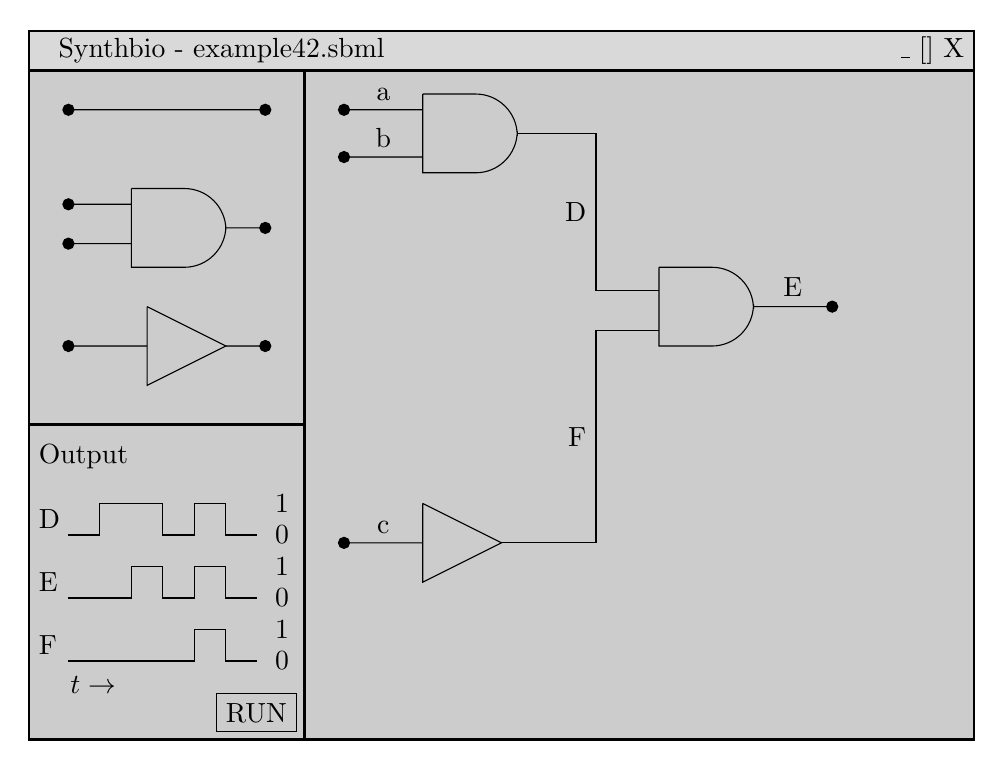
\begin{tikzpicture}

%main window
\draw[fill=black!20,line width=1] (-6,4) rectangle (6, -5);

% window title bar
\draw[fill=black!15,line width=1] (-6,4) rectangle (6, 3.5);
\node [anchor=west] at (-5.75, 3.75) {Synthbio - example42.sbml};
\node [anchor=east] at (6, 3.75) {\_ [] X};

% sidebar
\draw[fill=black!20,line width=1] (-6, 3.5) rectangle (-2.5, -5);
\draw[line width=1] (-6, -1) -- (-2.5, -1);

% wire
\draw (-5.5, 3) [fill]circle (2pt) -- ++( 2.5, 0) circle (2pt);

%and
\draw (-4.7, 2) [rounded corners=15pt] --  ++(1.2, 0)  -- ++(0, -1) [sharp corners] -- ++(-1.2, 0) -- ++(0, 1);
\filldraw (-5.5, 1.8) circle (2pt) -- (-4.7, 1.8);
\filldraw (-5.5, 1.3) circle (2pt) -- (-4.7, 1.3);
\filldraw (-3.5, 1.5) -- (-3, 1.5) circle (2pt);

%not
\draw (-4.5, 0.5) --  ++(1, -0.5) -- ++(-1, -.5) -- ++(0, 1);
\draw (-5.5, 0) [fill] circle (2pt) -- ++(1,0);
\draw (-3.5, 0) -- ++(.5, 0) [fill] circle (2pt);

%output
\node [anchor=west] at ( -6, -1.4) {Output};
\node [anchor=west] at(-5.6, -4.3) {$t \to$};

%signal D
\node [anchor=west] at ( -6, -2.2) {D};
\node [anchor=west] at ( -3, -2) {1};
\node [anchor=west] at ( -3, -2.4) {0};
\draw (-5.5, -2.4) -- ++(.4, 0) -- ++(0, .4) -- ++ (0.8, 0) -- ++(0, -.4) -- ++(.4, 0) -- ++(0, .4) -- ++(.4, 0) -- ++(0, -.4) -- ++(.4, 0);

%signal E
\node [anchor=west] at ( -6, -3) {E};
\node [anchor=west] at ( -3, -2.8) {1};
\node [anchor=west] at ( -3, -3.2) {0};
\draw (-5.5, -3.2) -- ++(.8, 0) -- ++(0, .4) -- ++ (0.4, 0) -- ++(0, -.4) -- ++(.4, 0) -- ++(0, .4) -- ++(.4, 0) -- ++(0, -.4) -- ++(.4, 0);

%signal F
\node [anchor=west] at ( -6, -3.8) {F};
\node [anchor=west] at ( -3, -3.6) {1};
\node [anchor=west] at ( -3, -4) {0};
\draw (-5.5, -4) -- ++(1.6, 0) -- ++(0, .4) -- ++ (0.4, 0) -- ++(0, -.4) --  ++(.4, 0);

%run button
\node [draw, anchor=south east] at (-2.6, -4.9) {RUN};

% Working area

%and gate
\draw (-2, 3) [fill]circle (2pt) -- node[above]{a} ++(1, 0);
\draw (-2, 2.4) [fill]circle (2pt) --node[above]{b} ++(1, 0);
\draw (-1, 3.2) [rounded corners=15pt] --  ++(1.2, 0)  -- ++(0, -1) [sharp corners] -- ++(-1.2, 0) -- ++(0, 1);

%signal B
\draw (0.2, 2.7) -- ++ (1, 0) -- node[left] {D} ++(0, -2) -- ++(.8, 0);

%another gate
\draw (2, 1) [rounded corners=15pt] --  ++(1.2, 0)  -- ++(0, -1) [sharp corners] -- ++(-1.2, 0) -- ++(0, 1);

\draw (3.2, .5) -- node[above] {E} ++(1, 0) [fill] circle (2pt);

%not gate
\draw (-2, -2.5) [fill]circle (2pt) -- node[above]{c} ++(1, 0);
\draw (-1, -2) --  ++(1, -0.5) -- ++(-1, -.5) -- ++(0, 1);

% signal C
\draw (0, -2.5) -- ++(1.2, 0) -- node[left] {F} ++(0, 2.7) -- ++ (.8, 0);

\end{tikzpicture}
